% arara: pdflatex: { synctex: yes }
% arara: makeindex: { style: ctuthesis }
%% arara: bibtex

%\listfiles


%\PassOptionsToPackage{cp1250}{inputenc}

% The class takes all the key=value arguments that \ctusetup does,
% and couple more: draft and oneside
\documentclass[twoside]{ctuthesis}

\makeatletter
\edef\mytoday{\expandafter\@gobbletwo\the\year\ifnum\month<10 0\fi\the\month\ifnum\day<10 0\fi\the\day}
\makeatother

% LaTeX logo with better kerning in sf bf font
\makeatletter
\newcommand\LaTeX@lmss@bx{L\kern -.33em{\sbox \z@ T\vbox to\ht \z@ {\hbox {\check@mathfonts \fontsize \sf@size \z@ \math@fontsfalse \selectfont A}\vss }}\kern -.15em\TeX}
\DeclareRobustCommand\myLaTeX{%
	\ifcsname LaTeX@\f@family @\f@series\endcsname
		\csname LaTeX@\f@family @\f@series\endcsname
	\else
		\LaTeX
	\fi
}

\usepackage{datetime}

\ctusetup{
%	preprint = {\ctuverlog \\ ctuman \mytoday},
	mainlanguage = czech,
	titlelanguage = czech,
	otherlanguages = {english, czech},
	title-czech = {Následování člověka mobilním robotem},
	title-english = {Following of Human by Mobile Robot},
	doctype-czech = {Bakalářská práce},
	doctype-english = {},
	xfaculty = F3,
	department-czech = {Katedra kybernetiky},
	department-english = {Department of Cybernetics},
	author = {Mykhaylo Zelenskyy},
	supervisor = {Ing. Jan Chudoba},
%	supervisor-address = {Ústav X, \\ Uliční 5, \\ Praha 99},
	keywords-czech = {robotika, počítačové vidění, řízení robotu},
	keywords-english = {robotics, computer vision, robot control},
	day = \the\day,
	month = \the\month,
	year = \the\year,
%	list-of-figures = false,
%	list-of-tables = false,
%	monochrome = true,
%	savetoner = true,
	pkg-listings = true,
	ctulstbg = none,
%	layout-short = true,
%	pkg-hyperref = false,
}

\ctuprocess

% Theorem declarations, this is the reasonable default, anybody can do what they wish.
% If you prefer theorems in italics rather than slanted, use \theoremstyle{plainit}
\theoremstyle{plain}
\newtheorem{theorem}{Theorem}[chapter]
\newtheorem{corollary}[theorem]{Corollary}
\newtheorem{lemma}[theorem]{Lemma}
\newtheorem{proposition}[theorem]{Proposition}

\theoremstyle{definition}
\newtheorem{definition}[theorem]{Definition}
\newtheorem{example}[theorem]{Example}
\newtheorem{conjecture}[theorem]{Conjecture}

\theoremstyle{note}
\newtheorem*{remark*}{Remark}
\newtheorem{remark}[theorem]{Remark}

\DeclareMathOperator{\atantwo}{atan2}

% Marginpars used as navigation aids.
\usepackage{mparhack}
\usepackage{epstopdf}
\usepackage{subfig}
\usepackage{siunitx}
\usepackage{url}


\newcommand\indexmp[1]{{\sffamily\bfseries#1}}

\ExplSyntaxOn
\cs_new:Nn \ctuman_domarginpar:n {
	\marginpar
	[ \raggedleft \footnotesize \sffamily #1 ]
	{ \raggedright \footnotesize \sffamily #1 }
}
\cs_generate_variant:Nn \ctuman_domarginpar:n { x }
\DeclareDocumentCommand \ctump { m } {
	\clist_set:Nn \ctuman_temp_clist { #1 }
	\ctuman_domarginpar:x { \clist_use:Nnnn \ctuman_temp_clist { \\ } { \\ } { \\ } }
	\clist_map_inline:Nn \ctuman_temp_clist { \index{##1|indexmp} }
	\ignorespaces
}
\ExplSyntaxOff

% Abstract in Czech
\begin{abstract-czech}
\end{abstract-czech}

% Abstract in English
\begin{abstract-english}
\end{abstract-english}

% Acknowledgements / Podekovani
\begin{thanks}
\end{thanks}

% Declaration / Prohlaseni
\begin{declaration}
I declare that this work is all my own work and I have cited all sources I have
used in the bibliography.

\medskip

Prague, \monthinlanguage{second} \ctufield{day}, \ctufield{year}

\vspace*{2cm}

Prohlašuji, že jsem předloženou práci vypracoval samostatně, a že jsem uvedl veškerou použitou literaturu.

\medskip

V Praze, \ctufield{day}.~\monthinlanguage{title}~\ctufield{year}
\end{declaration}

\usepackage{url}

\usepackage{tabularx,array}

\usepackage{mathtools,amssymb}

% A savebox for typesetting listings in the titles
\newsavebox{\myboxa}

%\newcommand*\symbO{$\color{red}\bowtie$}
\newcommand*\symbO{\raisebox{0.5\height}{\scalebox{0.7}{\color{red}${\vartriangleright}\mkern-6mu{\vartriangleleft}$}}}
\newcommand*\symbM{\raisebox{0.5\height}{\scalebox{0.7}{\color{red}${\blacktriangleright}\mkern-6mu{\blacktriangleleft}$}}}
\newcommand*\itemO{\item\leavevmode\kern-0.33em\symbO}
\newcommand*\itemM{\item\leavevmode\kern-0.33em\symbM}



\begin{document}



% We actually don't want inline listings to have a background color
\renewcommand \ctulstsep {0pt}

% \ctuclsname for typesetting the class' name
\newcommand\ctuclsname{\leavevmode\unhcopy\ctuclsnamebox}
\newsavebox\ctuclsnamebox
\begin{lrbox}{\ctuclsnamebox}
\ctulst!ctuthesis!
\end{lrbox}

\maketitle

\chapter{Úvod}

Pomocný robot se může zdát mnhým z nás jako futuristický sen. Takový robot by místo nás nosil věci, pomáhal při nákupech, asistoval v nemocnicích či ošetřoval raněné ve válkách.  Měl by tolik výhod, že by v budoucnu bylo trendem tohoto pomocníka vlastnit.

Bylo provedeno mnoho různých výzkumů ohledně návrhu robotů, které by dokázaly sledovat člověka. S tímto problémem jsou spojené dvě důležité otázky. Jaké senzory použit pro lokalizaci člověka? Jak řešit řízení a navigaci robotu tak, aby udržoval určitou vzdálenost a vyhýbal se případným překážkám?

Nejdříve je třeba definovat, co vlastně je robotem následující člověka. Jedná se o mobilního robota, který sleduje určitou osobu
a zároveň objíždí překážky a chová se k ostatním lidem jako k překážkám, tj. nezmění cíl sledování během jízdy.

Takový robot typicky může být vybaven mnoha různými senzory, např. laserovým, zvukovým nebo IR dálkoměrem, aby mohl měřit vzdálenost od překážek, kamerou pro detekci sledovaného objektu, bezdrátovým přenášečem signálu, GPS apod. Tyto senzory by měly fungovat současně, aby robot dokázal všechno, co se od něj očekává.

\section{Cíl práce}
Cílem této práce je navrhnout systém pro řízení robotu, tak aby dokázal splnit úkoly definované v úvodu. 

Při návrhu tohoto systému je třeba uvědomit si několik věcí:
\begin{enumerate}
	\item Cíl se nesmí pohybovat větší rychlostí, než je maximální rychlost robotu. Může se stát, že robot už nikdy nedokáže najít sledovaného člověka, dokud se dotyčný nevrátí na dostatečně blízko k robotu.

	\item Aby značka byla dobře detekovatelná, musí být umístěna v ochranném prostředí, tj. být kontrastní v porovnání s pozadím.

	\item V případě použití dálkoměru pro měření vzdálenosti mezi objekty je důležité, aby systém nedetekoval sledovaný cíl jako překážku.
\end{enumerate}

\section{Motivace}

Jak již bylo řečeno, robot s podobnou funkcionalitou by byl velice užitečný jako pomocník v různých oborech lidské činnosti. V medicínských zařízeních a domovech pro seniory by se takový robot mohl starat o pacienty (viz obr. \ref{rnc}), také by našel své uplatnění v armádě, kde by pomáhal vojákům s převozem nákladů. Vylepšená varianta robota by mohla posloužit jako tělesná stráž.


\begin{figure}
	\caption{Robot následující člověka}

	\label{rnc}
	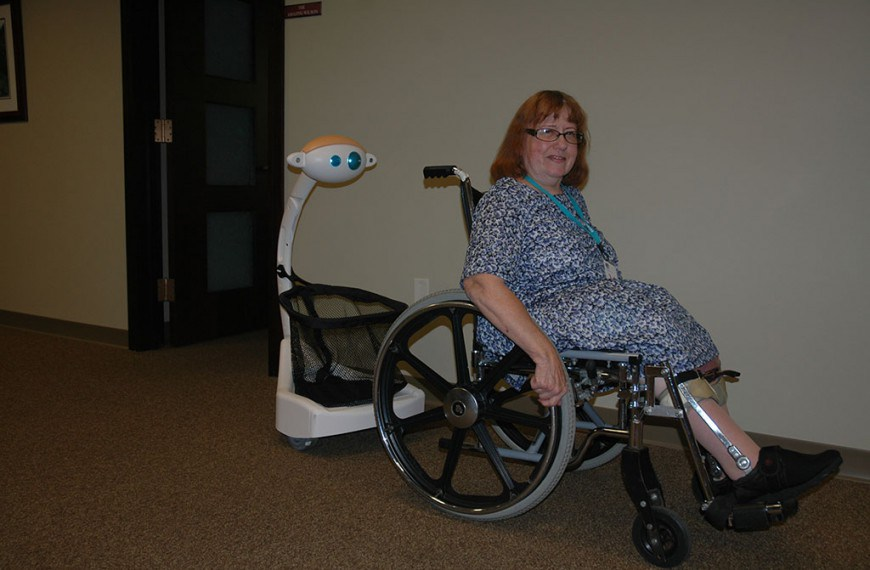
\includegraphics[width=\textwidth]{images/0/maxresdefault.jpg}
\end{figure}



\chapter{Návrh systému}

%https://pdfs.semanticscholar.org/85b3/0c6cf6853fed8f45502bd03cc85c3e2a59df.pdf
%https://agrosy.cs.uni-kl.de/fileadmin/Literatur/Braun05a.pdf
%Design and Development of Human Following Robot
Existuje několik výzkumných projektů, které se zabývají problematikou pomocných robotů, které by následovaly člověka. Většina těchto projektů zakládá na detekci pohybujícího se objektu, které je následně sledován. V některých pracích jsou použity neuronové sítě pro detekci obličeje a background subtraction pro nalezení pohybu v obraze \cite{cite:19}, např. pohybujících se nohou člověka. Avšak použití tohoto algoritmu vede k tomu, že sledovaný člověk musí být otočen k robotu obličejem, a prezence několika lidí v místnosti přivede k tomu, že robot nedokáže určit, koho musí následovat. V případě, že neuronová síť bude naučena pouze na konkrétního člověka, což by tento problém mohlo řešit, znovupoužitelnost algoritmu klesá, protože by bylo třeba síť přeučovat pro každý konkrétní případ.

Dalším možným řešením této problematiky je použití barevného markeru \cite{cite:18}, což znamená, že robot hledá určitou shodu barev, kterou pak sleduje. V tomto případě člověk může být otočen k robotu zády, a algoritmus může být použit i v plných lidí prostorech. Avšak detekce barevného vzoru nemusí být robustní kvůli změně osvětlení nebo špatné volbě barev, které nebudou dostatečně kontrastní v porovnání s oblečením sledovaného člověka.

Proto pro návrh této práce bylo rozhodnuto použít specifický druh vizuálních značek, což bude popsáno v následujícím textu. Cíl pro sledování musí být unikátní, a algoritmus detekce musí být robustní, aby nedocházelo k tomu, že robot nebude vědět, koho má sledovat. Robot dopředu bude vědět, jaký typ značky musí hledat, proto se snižuje šance, že si splete cíl s jiným člověkem nebo překážkou. 

\section{Volba vizuální značky}


%https://www.researchgate.net/publication/270107591_Visual_Localization_of_Mobile_Robot_Using_Artificial_Markers
%https://pdfs.semanticscholar.org/71e8/30b6da4b7adbfcd369664e5347a515e25d64.pdf
%http://www.uco.es/investiga/grupos/ava/sites/default/files/GarridoJurado2014.pdf
Mobilní robot bude následovat člověka, který má na sobě umístěnou předem známou vizuální značku. Pro navigaci robotu se v praxi běžně používají markery pro rozšířenou realitu \cite{cite:1}\cite{cite:2}\cite{cite:3}. Jejich detekce je většinou jednoduchá a můžou v sobě uchovávat užitečnou informaci, např. identifikační číslo, podle kterého robot pozná, koho sleduje. Jednu z možných vizuálních značek, které jsou v této práci použity, lze vidět na obrázku \ref{am}.

\begin{figure}[]
	\caption{Příklad vizuální značky}

	\label{am}
	
\includegraphics[width=0.5\textwidth]{images/2/ArucoMarker.jpg}
\end{figure}

\section{Volba souřadnicového systému}
\label{ss_section}

Pro řízení robotu je třeba zvolit souřadnicový systém, ve kterém se bude pohybovat.

Počátek zvolené souřadnicové soustavy umístěn do počáteční pozice robotu a osa X je ve stejném směru, jako počáteční směr jízdy robotu. Kladný směr jízdy robotu je v kladném směru osy Y, jak je vyobrazeno na \ref{ss}, a je v rozmezí $\left(-\pi; \pi\right)$. Poloha cíle (viz sekci \ref{mereni_polohy_cile}) je poté vztažená k poloze robotu a je počítána v čárkované soustavě, jejíž počátek je umístěn do aktuální pozice robotu, a je vůči původní otočená o $h$, kde $h$ je směr jízdy robotu.


\begin{figure}[H]
	\caption{Použitý souřadnicový systém}
	
	\label{ss}
	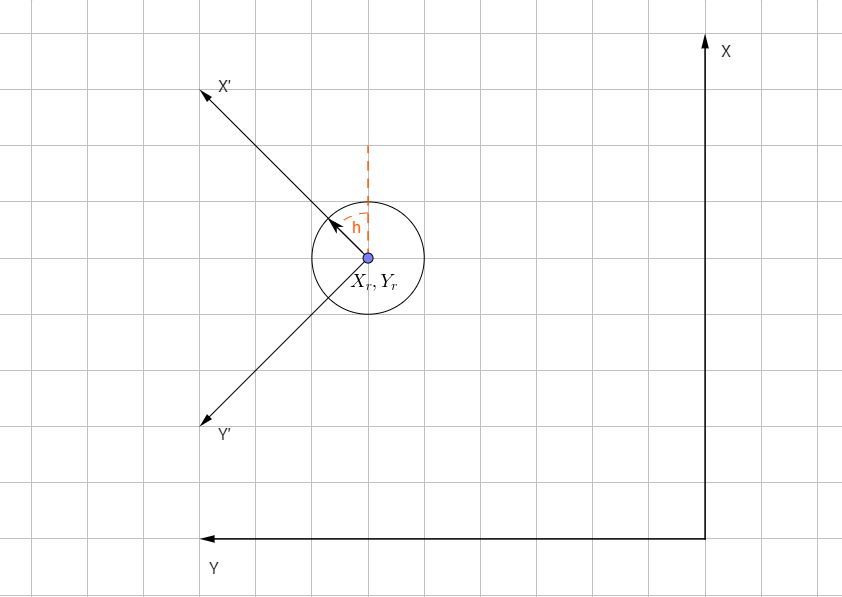
\includegraphics[width=0.9\textwidth]{images/2/ss.png}
\end{figure}
\section{Implementační záležitosti}

%http://opencv.org/about.html
%https://www.uco.es/investiga/grupos/ava/node/26

Protože se očekává, že běh software bude v reálném čase, musí být rychlý a stabilní. Z těchto důvodů bylo rozhodnuto, že bude použit jazyk C++.

Také v práci je použita knihovna OpenCV\cite{cite:4}, která nabízí obrovské možnosti pro zpracování obrazu. Tato knihovna obsahuje přes 2500 optimalizovaných algoritmů pro počítačové vidění a strojové učení. Některé z nich budou použity pro detekci vizuální značky ve výstupu z kamery. Navíc v této knihovně je implementován algoritmus pro detekci ArUco markeru \cite{cite:1}, který je podrobněji popsán v sekci \ref{aruco_marker}.

\chapter{Detekce}

\section{Zpracování obrazu z kamery}

Než bude možné použít rozpoznávací algoritmy, výstup z kamery musí být náležitě zpracován, aby odpovídal formátu, se kterým algoritmy pracují.

% http://citeseerx.ist.psu.edu/viewdoc/download?doi=10.1.1.420.7883&rep=rep1&type=pdf

%http://docs.opencv.org/trunk/d9/d8b/tutorial_py_contours_hierarchy.html

%http://docs.opencv.org/3.1.0/d5/dae/tutorial_aruco_detection.html

%https://en.wikipedia.org/wiki/Ramer–Douglas–Peucker_algorithm#cite_ref-1
Načtený snímek je převeden do černobílé podoby, je tedy použito prahování. Jelikož se předpokládá, že se robot může pohybovat v prostředí s nerovnoměrným osvětlením, pro binarizaci obrazu je vhodné použit adaptivní prahování \cite{cite:5} (viz obr. \ref{adapt}). Tato metoda počítá práh pro malé části obrazu místo globálního nastavení prahu pro celý snímek.

%https://pdfs.semanticscholar.org/55e6/6333402df1a75664260501522800cf3d26b9.pdf
Dále je třeba najít kontury. Cannyho algoritmus pro nalezení kontur je implementován v knihovně OpenCV. Tato funkce navíc zajišťuje zachování hierarchie kontur\cite{cite:6}, tedy topologii obrázku, jak je vidět na \ref{hierarch}. Tato informace je užitečné pro následné rozpoznávání, protože pak kontury na nejnižší nebo nejvyšší úrovni hierarchie můžou být ignorovány, pokud se předpokládá, že vizuální značka bude umístěna v ochranné zóně a bude obsahovat další pod-vzory.


\begin{figure}
	\caption{Příklad použití adaptivního prahování \cite{cite:5}}

	\label{adapt}
	\subfloat[Před prahováním]{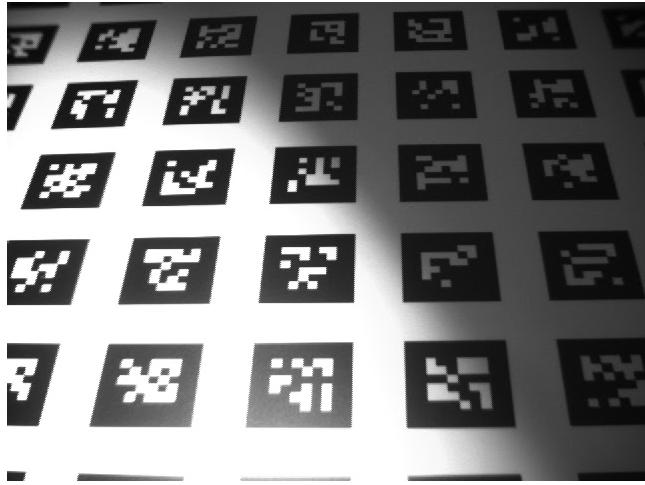
\includegraphics[width=0.45\textwidth]{images/2/adapt_1.jpg}}
	\hfill
	\subfloat[Po prahování]{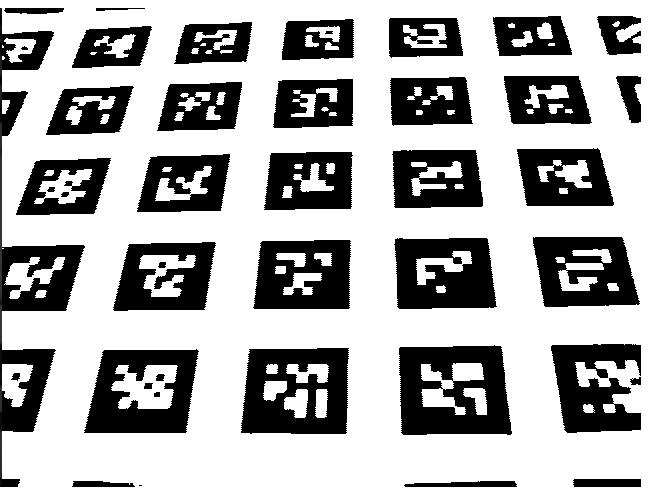
\includegraphics[width=0.45\textwidth]{images/2/adapt_2.jpg}}
\end{figure}

\begin{figure}

	\caption{Hierarchie (topologie) obrazu \cite{cite:6}}

	\label{hierarch}
	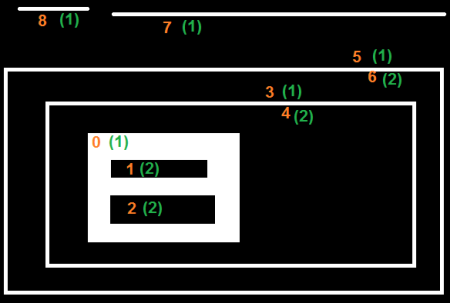
\includegraphics[width=0.8\textwidth]{images/2/ccomp_hierarchy.png}
\end{figure}

\section{Rozpoznávání vzoru}

%http://web.stanford.edu/class/ee368/Handouts/Lectures/2014_Spring/Combined_Slides/9-Template-Matching-Combined.pdf
%http://docs.adaptive-vision.com/4.7/studio/machine_vision_guide/TemplateMatching.html
Pro rozpoznávání vizuální značky je vhodné použít algoritmus, který zakládá na hledání známého vzoru v obraze. Nejběžnějším algoritmem, který se pro této účely používá, je Template Matching \cite{cite:16}. Podstatou tohoto algoritmu je to, že se pro různé velikosti vstupného obrazu počítá jeho korelace se známým vzorem. Vytváří se tzv. pyramida obrazů \cite{cite:17}, která se skládá ze vstupních obrázků různé velikosti a orientace. Každý obraz v této pyramidě je rozdělen na oblasti o stejné velikosti, jako je velikost vzoru. Pro každou z těchto oblasti se výpočte korelace se vzorem. Následně je zvolena oblast, kde je korelační koeficient největší.

Kvůli tomu, že korelace musí být spočtena pro velký počet vstupních obrazu o různé velikosti, Template Matching může být pomalý. Jelikož se předpokládá použití čtvercové vizuální značky, je praktičtější nejdříve najít oblast zájmu (Region of Interest, ROI), pro níž se spočte korelace se známým vzorem.

Proto pro detekci vizuální značky byl navržen korelační algoritmus, který je popsán v následujícím textu. Pro porovnání funkčnosti tohoto algoritmu byl použit ArUco marker detektor  \cite{cite:7}, který je k dispozici přímo v knihovně OpenCV.

\subsection{Korelační algoritmus}

Tento algoritmus využívá principu korelaci mezi dvěma veličinami, tedy mezi známým vzorem a nalezenou ROI. Korelace uvádí, jak jsou na sobě tyto veličiny závislé, a může nabývat hodnot od -1 do +1. Hodnota korelačního koeficientu blížící se -1 značí nepřímou závislost veličin, koeficient blízký +1 naopak značí přímou závislost, což je zobrazeno na \ref{korelace}.

\begin{figure}

	\caption{Příklad korelace mezi markery vůči referenčnímu}

	\label{korelace}
	\subfloat[Referenční marker]{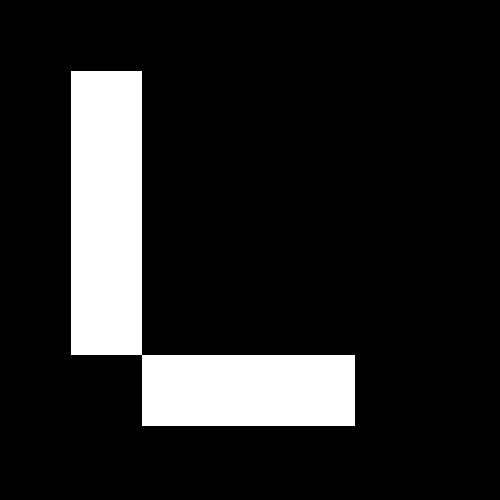
\includegraphics[width=0.4\textwidth]{images/2/3.jpg}}
	\hfill
	\subfloat[cor($I_1, I_2$) = 0.47]{
\includegraphics[width=0.4\textwidth]{images/2/682_klad.jpg}}
	\hfill
	\subfloat[cor($I_1, I_2$) = -0.55]{
\includegraphics[width=0.4\textwidth]{images/2/3_zap.jpg}}
	\hfill
	\subfloat[cor($I_1, I_2$) = -0.04]{
\includegraphics[width=0.4\textwidth]{images/2/682_zadna.jpg}}
\end{figure}
Hledaná ROI je v zjednodušeném případě konvexní čtyřúhelník, proto stačí s použitím informace o topologii obrazu spočítat polygony nalezených kontur a vybrat pouze ty, co obsahují čtyři strany a nejsou konkávní. Pro aproximaci křivky se používá Ramerův Douglasův Peuckerův algoritmus \cite{cite:8} (viz obr. \ref{approx}), který je již implementován v OpenCV.
\begin{figure}

	\caption{Aproximace křivky pomocí Ramerova Douglasova Peuckerova algoritmu}

	\label{approx}
	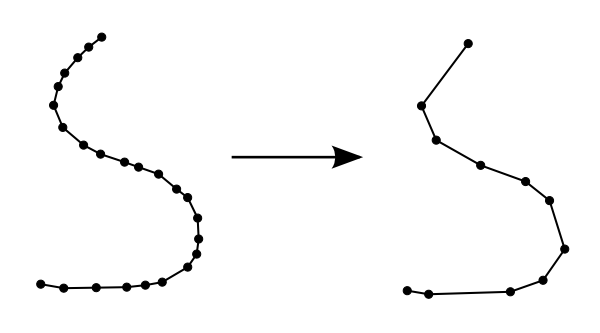
\includegraphics[width=0.8\textwidth]{images/2/approx.png}
\end{figure}


Následně je spočítána transformační matice mezi nalezeným polygonem a známým vzorem. Pomocí této matice se polygon převede do takové podoby, aby byl porovnatelný se vzorem.

Dále dojde k vyhodnocení korelace nalezené ROI a vzoru. Pokud je vypočtený korelační koeficient větší, než zadaný práh, ROI se vyhodnotí jako správně označena a algoritmus vrátí souřadnice jejích rohů pro následné zpracování.

Korelaci mezi dvěma obrázky $I_1$ a $I_2$ s $N$ pixely je vypočtena následujícím způsobem:

	\begin{equation}
	\mu_{1,2} = \frac{\sum_{i,j}I_{i,j}}{N},
	\end{equation}
	\begin{equation}
	\sigma_{1,2} = \sqrt{\left(\frac{\sum_{i,j}(I_{i,j} - \mu_{1,2})^2}{N}\right)^2},
	\end{equation}
	\begin{equation}
	covar(I_1, I_2) = \frac{(I_1 - \mu_1)\cdot(I_2 - \mu_2)}{N},
	\end{equation}
	\begin{equation}
	cor(I_1, I_2) = \frac{covar(I_1, I_2)}{\sigma_1 \sigma_2}.
	\end{equation}

\subsection{ArUco marker detektor}
\label{aruco_marker}

Tento algoritmus je implementován v OpenCV knihovně a umožňuje rozpoznávání ArUco markerů nebo podobných vizuálních značek. Podobně jako výše uvedený korelační algoritmus, hledá konvexní čtyřúhelník. Rozdíl pak spočívá v odlišném zpracování nalezené ROI, kde se místo korelace využívá binární mapa kandidáta.

ROI je rozdělena na mřížku s počtem buněk rovným počtu bitů hledaného vzoru (viz obr. \ref{cell}). Následně se spočítá, kolik bílých a černých pixelů obsahuje každá buňka, na základě čehož se vyhodnotí, jestli buňka je černá nebo bílá (viz obr. \ref{cellm}). Pokud detektor ve svém slovníku obsahuje vzor se stejnou binární maskou, vrátí souřadnice rohů nalezené ROI.

\begin{figure}
	\caption{Buňky ArUco markeru}

	\label{cell}
	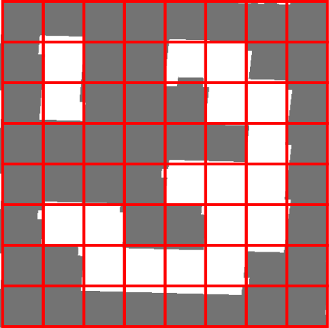
\includegraphics[width=0.5\textwidth]{images/2/bitsextraction1.png}
\end{figure}
\begin{figure}
	\caption{Vyhodnocení obrázku pomocí detektoru ArUco}

	\label{cellm}
	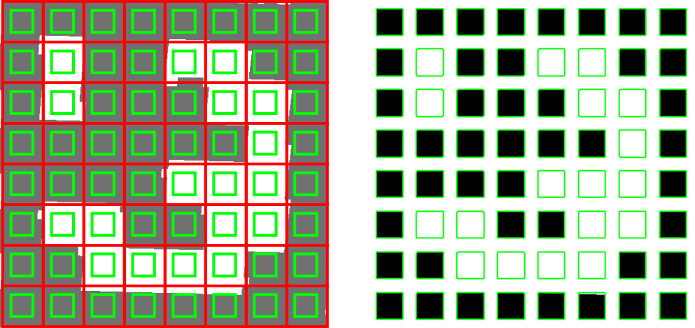
\includegraphics[width=1\textwidth]{images/2/bitsextraction2.png}
\end{figure}
\section{Měření polohy cíle}
\label{mereni_polohy_cile}
%http://www.huecandela.com/hue-x/pin-pdf/Prober-%20Wellman.pdf

Algoritmy popsané výše naleznou polohu vizuální značky v obraze, z čehož lze spočítat její umístění vůči kameře, je-li známa velikost této značky. Pro výpočty lze použít model ideální (dírkové) kamery \cite{cite:9}, kde vzdálenost mezi kamerou a značkou je vyjádřena jako

\begin{equation}
d = \frac{fX}{x},
\end{equation}

kde $x$ značí nejkratší vzdálenost mezi dvěma rohy nalezené značky, $f$ je ohnisková vzdálenost a $X$ je známá délka hrany značky .

Pro nalezení posunutí značky vůči kameře při odklonění od její osy musí být znám zorný úhel kamery. Ten lze spočítat dle vztahu

\begin{equation}
\alpha = 2\arctan\left(\frac{w}{2f}\right),
\end{equation}

kde $w$ je šířka výstupního obrazu z kamery.

Potom úhel, který pokrývá jeden pixel snímku, je vyjádřen vztahem

\begin{equation}
APP = \frac{\alpha}{w}.
\end{equation}

Následně posunutí objektu vůči středu kamery je

\begin{equation}
\phi = (x_c - x_t)APP,
\end{equation}

kde $x_c$ je pixel vyjadřující střed kamery v horizontálním směru, $x_t$ je pixel vyjadřující střed nalezené značky v horizontálním směru.

\begin{figure}
	\caption{Měřené veličiny $d$ a $\phi$}

	\label{mereni}
	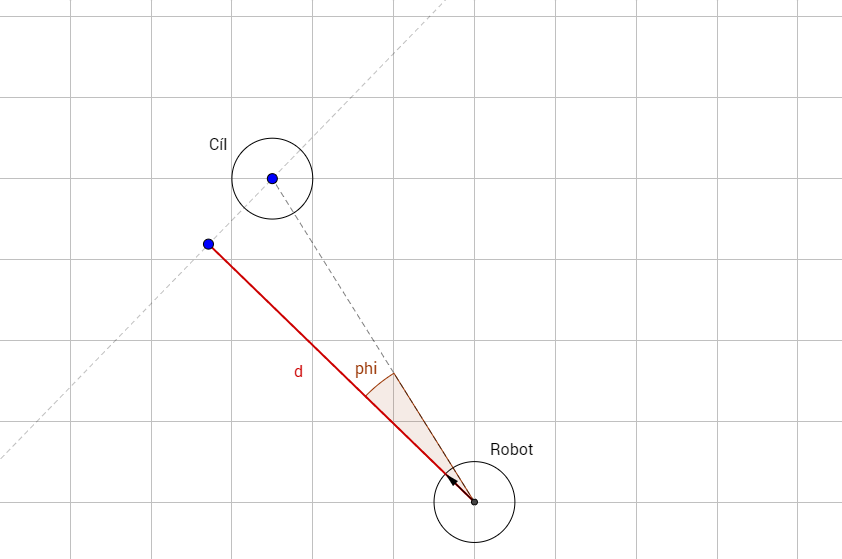
\includegraphics[width=1\textwidth]{images/2/mereni.png}
\end{figure}
\section{Kalmanův filtr}
\label{kalman_section}
%http://www.diss.fu-berlin.de/docs/servlets/MCRFileNodeServlet/FUDOCS_derivate_000000000473/2005_12.pdf

%https://github.com/rlabbe/Kalman-and-Bayesian-Filters-in-Python


Při sledování člověka může nastat situace, že vizuální značka nebude detekovatelná. Potom není možnost spočítat polohu značky vůči robotu, a tak robot buď zastaví, nebo bude pokračovat pohyb dle posledního měření. Toto může přivést k tomu, že se člověk bude muset vrátit k robotu, aby ten ho znovu začal sledovat. Aby tato situace nenastala, je je třeba predikovat polohu cíle z předchozích měření. Pro tyto účely je v práci použit Kalmanův filtr \cite{cite:10}.

Model lze popsat pomocí následujícího stavového vektoru:
\begin{equation}
{\boldsymbol{x}} =
\begin{bmatrix}
x&y&v_{x}&v_{y}
\end{bmatrix}^T,
\end{equation}

kde $v_{x}$, resp. $v_{y}$, značí rychlost ve směru osy X, resp. Y.


Stavový model je pak vyjádřen jako

\begin{equation}
\label{x_t+1}
{\boldsymbol{x}}_{t+1} = \boldsymbol{F}{\boldsymbol{x}}_{t},
\end{equation}

kde $\boldsymbol{F}$ je matice přechodu stavů $\boldsymbol{x}$ z času $t$ do času $t + 1$ a platí, že

\begin{equation}
\boldsymbol{F} = \begin{bmatrix}
1&0&1&0\\
0&1&0&1\\
0&0&dt&0\\
0&0&0&dt
\end{bmatrix}.
\end{equation}

Pro sledování cíle lze Kalmanův filtr rozdělit do tří kroků:

\textbf{1.  Inicializace ($t = 0$).} Během tohoto kroku je nastavena počáteční pozice cíle $\boldsymbol{x}_0$ a výchozí hodnota pro kovarianční matici $\boldsymbol{P}_0$. Jelikož počáteční pozice cíle nemusí být známa, je vhodné zvolit $\boldsymbol{x}_0$ tak, aby v případě, že kamera nedetekuje značku po první iteraci, zůstával robot na místě.

\textbf{2. Predikce ($t > 0$).} V tomto kroku se provádí predikce polohy cíle v čase $t + 1$, tj. $\boldsymbol{x}_{t+1}$, dle \ref{x_t+1}. Také se počítá nová kovarianční matice dle následujícího vztahu

\begin{equation}
\boldsymbol{P}_{t+1} = \boldsymbol{F}\boldsymbol{P}_t\boldsymbol{F}^T + \boldsymbol{Q}_{t+1},
\end{equation}

kde $\boldsymbol{Q}$ značí matici kovariancí šumů (výpočet viz \cite{cite:11}).

\textbf{3. Filtrace ($t > 0$).} Během tohoto kroku je poloha cíle upřesněna na základě provedeného měření. Nejdříve se spočte rozdíl mezi reálnou polohou a predikovanou v kroku 2.:

\begin{equation}
\boldsymbol{y}_{t} = \begin{bmatrix}
x_{m_t}\\y_{m_t}
\end{bmatrix} - \boldsymbol{H}\boldsymbol{x}_t,
\end{equation}

kde

\begin{equation}
\boldsymbol{H} = \begin{bmatrix}
1&0&0&0\\
0&1&0&0
\end{bmatrix}.
\end{equation}

Dále se vypočítá Kalmanovo zesílení, pro nějž platí:

\begin{equation}
\boldsymbol{K}_t = \boldsymbol{P}_t\boldsymbol{H}^T(\boldsymbol{H}\boldsymbol{P}_t\boldsymbol{H}^T + \boldsymbol{R})^{-1},
\end{equation}

kde $\boldsymbol{R}$ ja matice kovariancí šumů (výpočet viz \cite{cite:11}).

Následně se provede zpřesnění polohy cíle a aktualizuje se kovarianční matice:

\begin{equation}
\boldsymbol{x}_{t+1} = \boldsymbol{x}_t + \boldsymbol{K}_t\boldsymbol{y}_t,
\end{equation}

\begin{equation}
\boldsymbol{P}_{t+1} = (\boldsymbol{I} - \boldsymbol{K}_t\boldsymbol{H})\boldsymbol{P}_t.
\end{equation}

Celý proces lze shrnout pomocí diagrame \ref{kalman_diag}.
\begin{figure}[H]
	\caption{Shrnutí algoritmu Kalmanova filtru}

	\label{kalman_diag}
	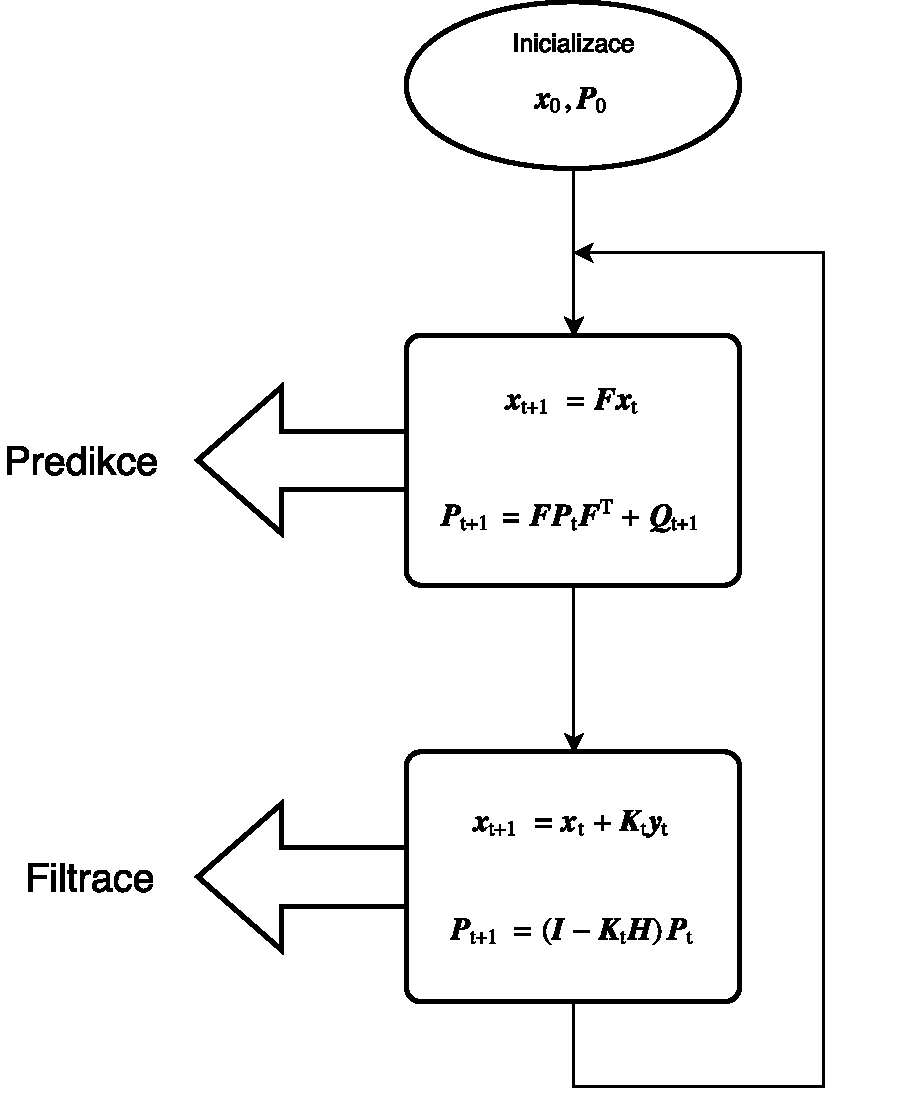
\includegraphics[width=0.7\textwidth, height=0.7\textwidth]{images/2/kalman_diagram.pdf}
\end{figure}
Z nalezených hodnot $x$ a $y$ lze jednoduše odvodit hodnoty $d$ a $\phi$, což je také vidět na \ref{inv}. Jelikož se předpokládá, že poloha robotu je známa, lze spočítat $x_t$ a $y_t$, což je poloha cíle vůči robotu, jako:

\begin{equation}
x_t = x - x_r,
\end{equation}

\begin{equation}
y_t = y - y_r.
\end{equation}

Dále jsou pak $\phi$ a $d$ nalezeny dle vztahů:

\begin{equation}
\phi = h - \atantwo(y_t, x_t),
\end{equation}

\begin{equation}
d = \sqrt{x_t + y_t}\cos(\phi).
\end{equation}
\begin{figure}
	\caption{Odvození hodnot $d$ a $\phi$ ze známé polohy cíle}

	\label{inv}
	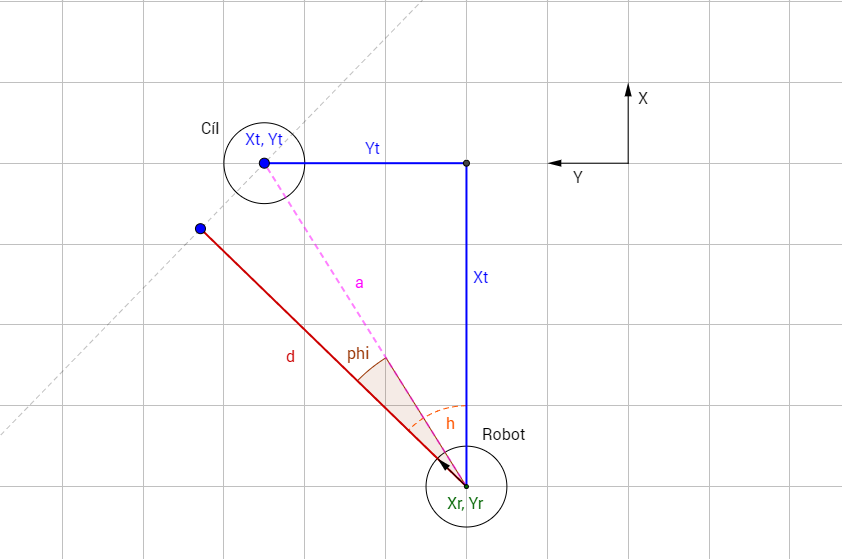
\includegraphics[width=1\textwidth]{images/2/neco.png}
\end{figure}
\chapter{Řízení robotu}

\section{Vyhýbání se překážkám}

Pro řízení autonomního robotu je důležité, aby se během sledování cíle dokázal vyhýbat překážkám. Algoritmů pro řízení robotu v prostředí s překážkami je několik \cite{cite:20}, jejichž přehled je k nalezení v příloze \ref{obstacle_avoidance}.

Jelikož se předpokládá, že robot bude řízen v relativní souřadnicově soustavě a není možnost vždy mít přesné globální souřadnice robotu a překážek, je třeba zvolit takový algoritmus, který by spoléhal pouze na lokální mapu prostředí, která by se vytvářela z měření dálkoměru. Dalším omezením pro výběr algoritmu je popis modelu robotu. 

\subsection{Vector Field Histogram (VFH)}

%http://www-personal.umich.edu/~johannb/Papers/paper16.pdf

%http://www.imavs.org/papers/2016/62_IMAV2016_Proceedings.pdf


Princip tohoto algoritmu \cite{cite:12} spočívá v tom, že se na základě dat naměřených dálkoměrem vytvoří lokální mřížková mapa prostředí o poloměru $r_{map}$. Každá buňka této mapy tak obsahuje hodnotu obsazenosti odpovídající oblasti v reálném světě (viz obr. \ref{mrizka}). Z této mapy se následně spočítá polární histogram, podle kterého se určí směr jízdy robotu.

\begin{figure}
	\caption{Lokální mapa prostředí o poloměru $r_{map}$ = 10}

	\label{mrizka}
	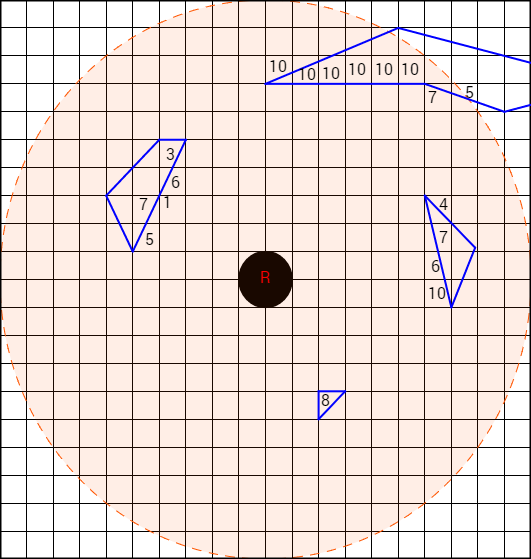
\includegraphics[width=0.6\textwidth, height = 0.6\textwidth]{images/3/mrizka.png}
\end{figure}

Celý proces tímto způsobem můžeme rozdělit na tři kroky: vytvoření primárního polárního histogramu, prahování primárního histogramu (vytvoření binární reprezentace), a nakonec výběr kandidátů pro směr pohybu.

\subsubsection{Primární polární histogram}

Polární histogram je rozdělen na sektory tak, aby každý z nich odpovídal úhlu $\alpha$, který je volen takovým způsobem, aby $\frac{360}{\alpha}$ bylo celé číslo. Tedy například pro $\alpha = 15^{\circ}$ histogram obsahuje 24 sektorů (viz obr. \ref{polar}).

Pro každou buňku aktivního regionu, tedy lokální mapy vytvořené kolem robotu, se spočte směr, ve kterém se vůči středu nachází, a její význam.
Směr je spočítán dle vztahu:

\begin{equation}
\beta_{i,j} = 	\atantwo ( y_o - y_i, x_o - x_i),
\end{equation}

kde $x_o, y_o$ značí souřadnice střed mapy, $x_i, y_i$ jsou souřadnice buňky.

Dále pak významnost buňky je:

\begin{equation}
m_{i,j} = c_{i,j}^2(a - bd_{i,j}^2),
\end{equation}

kde $c_{i,j}$ je obsazenost buňky a $d_{i,j}$ vzdálenost buňky od pozice robotu.

Parametry $a$ a $b$ jsou voleny dle vztahu:

\begin{equation}
a - b\left(\frac{r_{map} - 1}{2}\right)   = 1.
\end{equation}


Aby robot nejel blízko k okrajům překážek, zavádí se kompenzace jeho velikosti pomocí poloměru robotu $r_{rob}$ a minimální povolené vzdálenosti mezi robotem a překážkou $d_{safety}$:

$$\gamma_{i,j} = \arcsin\left(\frac{r_{rob} + d_{safety}}{d_{i,j}}\right)$$
Histogram je potom spočten vztahem:

\begin{equation}
H_k^p = \sum_{i,j \in C_{\alpha} } m_{i,j}h_{i,j},
\end{equation}

kde

$$h_{i,j} = \left\{
\begin{array}{ll}
1&\textrm{jestli $k\alpha \in \left[\beta_{i,j} - \gamma_{i,j}; \beta_{i,j} + \gamma_{i,j}\right]$,} \\
0&\textrm{jinak.}
\end{array}
\right.
$$


\begin{figure}
	\caption{Polární histogram s vyobrazenými prahy $\tau_{low}$ (zeleně) a $\tau_{high}$ (fialově)}

	\label{polar}
	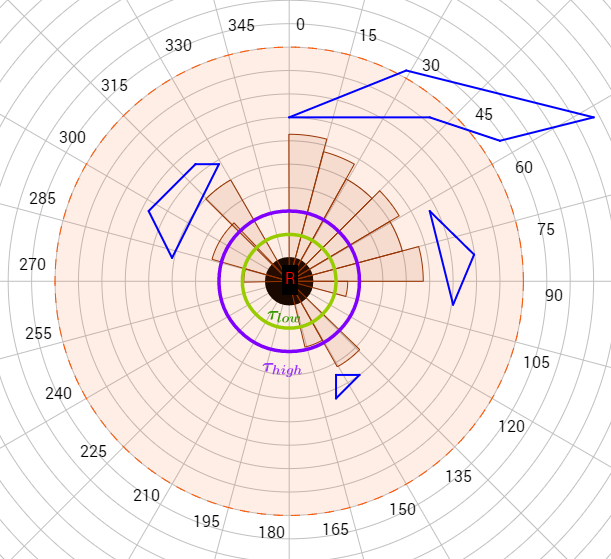
\includegraphics[width=0.8\textwidth]{images/3/polar.png}
\end{figure}
\subsubsection{Binární polární histogram}

Aby bylo možné určit kandidáty pro další směr pohybu, primární histogram musí být převeden do binární podoby.

$$H_{k,i}^{b} = \left\{
\begin{array}{ll}
1&\textrm{jestli $H_{k,i}^p > \tau_{high}$,}\\
0&\textrm{jestli $H_{k,i}^p < \tau_{low}$,}\\
H_{k, i-1}^b&\textrm{jinak.}
\end{array}
\right.
$$

\subsubsection{Výběr kandidátů}

Kandidáty pro nový směr pohybu se volí dle toho, do jaké kategorie je zařazeno volné místo v binárním histogramu. Ty průjezdy, které mají velikost (tedy vzdálenost mezi pravým okrajem $k_r$ a levým $k_l$) menší, než $s_{max}$, se nazývají úzké, jiné jsou naopak nazývány široké.

Pro úzké průjezdy lze zvolit pouze jednoho kandidáta, a to:

$$\begin{array}{ll}
c_n = \frac{k_r + k_l}{2}&\textrm{centrální sektor}
\end{array}$$

Široké průjezdy mají tři možné kandidáty:

$$\begin{array}{ll}
c_r = k_r + \frac{s_{max}}{2}&\textrm{pravý sektor,}\\

c_l = k_l - \frac{s_{max}}{2}&\textrm{levý sektor,}\\

c_t = k_t&\textrm{pokud $k_t \in \left[c_r;c_l\right]$}
\end{array}$$

Nový směr pohybu se zvolí dle minimální ceny spočítané pro kandidáta $c_i$ pomocí vztahu \cite{cite:13}

\begin{equation}
g(c_i) = \mu_1 \Delta\left(c_i, k_t\right) + \mu_2\Delta\left(c_i, \frac{h}{\alpha}\right) + \mu_3\Delta\left(c_i, k_{d, n-1}\right)
\end{equation}

přičemž $k_{d, n-1}$ je minule zvolený kandidát,
$\mu_1, \mu_2, \mu_3$ jsou konstanty, zvolené dle vztahu $\mu_1 > \mu_2 + \mu_3$ a také platí, že

\begin{equation}
\Delta(c_1, c_2) = \min\left\{|c_1 - c_2|, |c_1 - c_2 - \frac{360^{\circ}}{\alpha}|, |c_1 - c_2 + \frac{360^{\circ}}{\alpha}|\right\}
\end{equation}


\section{PID regulátor}

%https://www.cs.hmc.edu/~dodds/projects/RobS05/XPort/XPortArticle.pdf

Za jízdy je třeba, aby byla mezi robotem a cílem udržována určitá vzdálenost $d$ a hodnota úhlu $\phi$ byla co nejmenší, nejlépe nulová. Pro tyto účely je navržen PID regulátor  \cite{cite:14}, který pro aktuální odchylku od referenčních bodů spočte dopřednou a úhlovou rychlost, které se následně převedou na rychlosti motorů. Zjednodušený nákres algoritmu je zobrazen na \ref{pid}.  Pokud je $\epsilon_d$, resp. $\epsilon_\phi$, v pásmu $\left[-\epsilon_{d_0}; \epsilon_{d_0}\right]$, resp. $\left[-\epsilon_{\phi_0}; \epsilon_{\phi_0}\right]$, pak bude výstup PID regulátoru nulový. Jinak je od odchylky odečtena hodnota $\epsilon_{d_0}$, resp. $\epsilon_{\phi_0}$, což zaručí to, že robot nebude kmitat na místě, pokud bude blízko referenčního bodu, a řízení bude plynulé.

\begin{figure}
	\caption{PID regulace}

	\label{pid}
	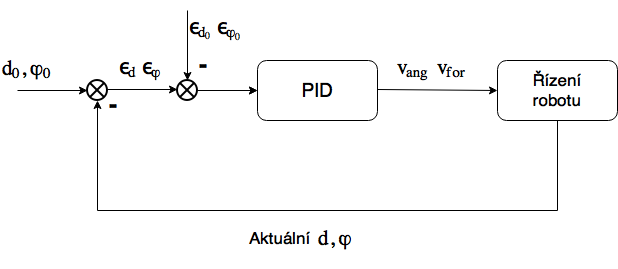
\includegraphics[width=0.9\textwidth, height = 0.4\textwidth]{images/3/PID.png}
\end{figure}


\chapter{Simulace}
\label{simulace}
%http://www.coppeliarobotics.com/index.html

Pro simulaci byl zvolen simulátor V-Rep \cite{cite:15}. V tomto prostředí byly vytvořeny dva roboty: jeden s vizuální značkou, druhý vybaven kamerou a laserovým dálkoměrem sledoval prvního (viz obr. \ref{robots}). Robot s vizuální značkou je řízen uživatelem pomocí klávesnice. Referenční vzdálenost mezi dvěma roboty byla zvolena \SI{1}{\meter}, požadovaná odchylka vizuální značky od středu kamery \SI{0}{\radian}. Maximální dopřední rychlost obou robotů byla nastavena na \SI{2.5}{\meter\per\second}

\begin{figure}
	\caption{Roboty vytvořené v simulátoru V-Rep}

	\label{robots}
	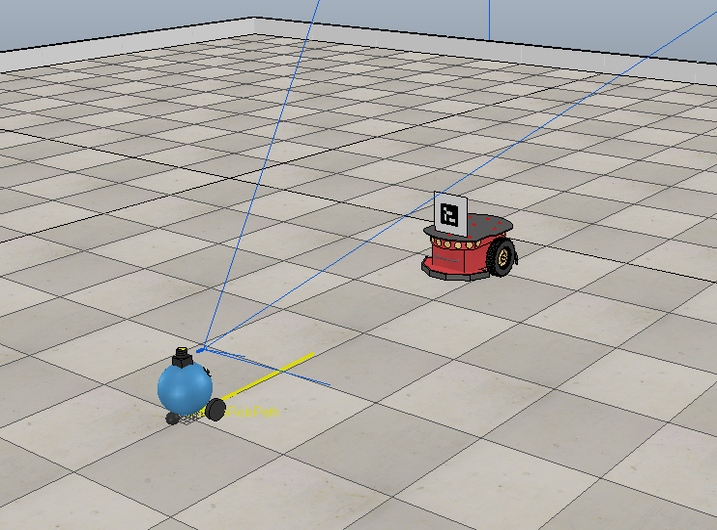
\includegraphics[width=0.8\textwidth]{images/5/robots.png}
\end{figure}
\section{Porovnání algoritmů detekce}

Oba algoritmy byly porovnávány při použití značky o velikosti 10x10 \SI{}{cm} a rozlišením kamery 512x512 pixelů. Bylo porovnáno několik parametrů, a to maximální vzdálenost, na které je vizuální značka ještě detekovatelná, stabilní vzdálenost, při které je značka detekována bez přerušení. Dále byl porovnán maximální a stabilní úhel otočení vizuální značky vůči robotu a také průměrný výpočetní čas na jednu iteraci algoritmu. Výsledky jsou znázorněny v tabulce \ref{porovnani}. Je patrné, že detekční schopnosti korelačního algoritmu jsou poněkud horší, než u ArUco detektoru. Avšak je třeba zdůraznit, že ArUco detektor sice dokázal rozpoznat vizuální značku na vzdálenosti přes 5 metrů od kamery, úspěšnost detekcí na tak velké vzdálenosti byla podprůměrná, přibližně 40 \%. Co se týká úhlu otočení značky vůči robotu, tam se korelační algoritmus ukázal být lepší a stabilně detekuje značku při 60$^\circ$ otočení. ArUco má na hranicích detekovatelnosti, tj. při 70$^\circ$ otočení, pouze 15\% úspěšnost.

\begin{table}[hbt]
	\centering
	\caption{Porovnání korelačního algoritmu a ArUco detektoru}
	\label{porovnani}
	\begin{tabular}{|c|c|c|}
		\hline
		Název algoritmu              & Korelační algoritmus & ArUco detektor \\ \hline
		Max. vzdálenost {[}m{]}      & 3.5                 & 5.4           \\ \hline
		Stabilní vzdálenost {[}m{]}  & 3.5                 & 3.8           \\ \hline
		Max. úhel {[}$^\circ${]}     & 60                   & 70             \\ \hline
		Stabilní úhel {[}$^\circ${]} & 60                   & 55             \\ \hline
		Výpočetní doba {[}ms{]}      & 15                   & 15             \\ \hline
	\end{tabular}
\end{table}
Hlavní rozdíl mezi těmito algoritmy spočívá v možnostech jejich využití. Zatímco ArUco detektor je zaměřený pouze na ArUco markery, korelační algoritmus je obecnější a dá se použít na jakýkoliv typ vizuální značky. ArUco detektor umožňuje přidání dalších značek do své knihovny, ale jedná se pouze o binární obrázky podobné znázorněnému na obr. \ref{aruco_marker}. Korelační algoritmus by měl detekovat i značku, kterou nelze reprezentovat jako bit-mapu, viz např. obr. \ref{hiro}.


\begin{figure}[H]
	\caption{Příklad značky pro korelační algoritmus}

	\label{hiro}
	
\includegraphics[width=0.5\textwidth]{images/5/r1301.jpg}
\end{figure}

\section{Porovnání naměřených a reálných hodnot}

\begin{figure}[hbt]
	\caption{Poloha sledovaného objektu během simulace}

	\label{sled}
	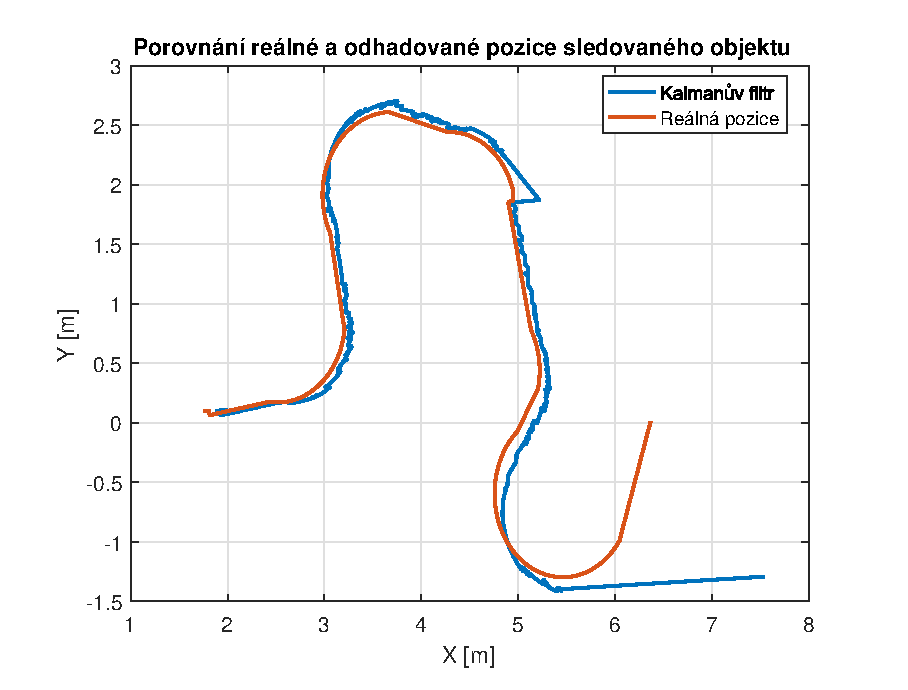
\includegraphics[width=0.8\textwidth]{images/5/pos_pioner.eps}
\end{figure}

Jelikož se v implementovaném programu provádí různé výpočty, je třeba porovnat, jakou mají tyto hodnoty odchylku vůči reálným. Kalmanův filtr, popsaný v \ref{kalman_section}, predikuje polohu cíle a v případě neúspěšné detekce vizuální značky je umístění sledovaného objektu vůči robotu odvozeno právě z predikované polohy. Na obrázku \ref{sled} lze vidět, že výpočet pomocí Kalmanova filtru skoro po celou dobu simulace odpovídá reálné poloze sledovaného objektu. Velká odchylka pak je až na konci simulace, kdy vizuální značka brzo zmizela ze zorného pole robotu a nebylo možné ji v krátké době najít. Toto také odpovídá výsledkům, které jsou na \ref{dist} a \ref{odch}, kde je vidět, že po cca 2000. iteraci je rozdíl mezi změřenými a reálnými hodnotami výrazný.


\begin{figure}[H]
	\caption{Vzdálenost mezi robotem a sledovaným objektem (d)}

	\label{dist}
	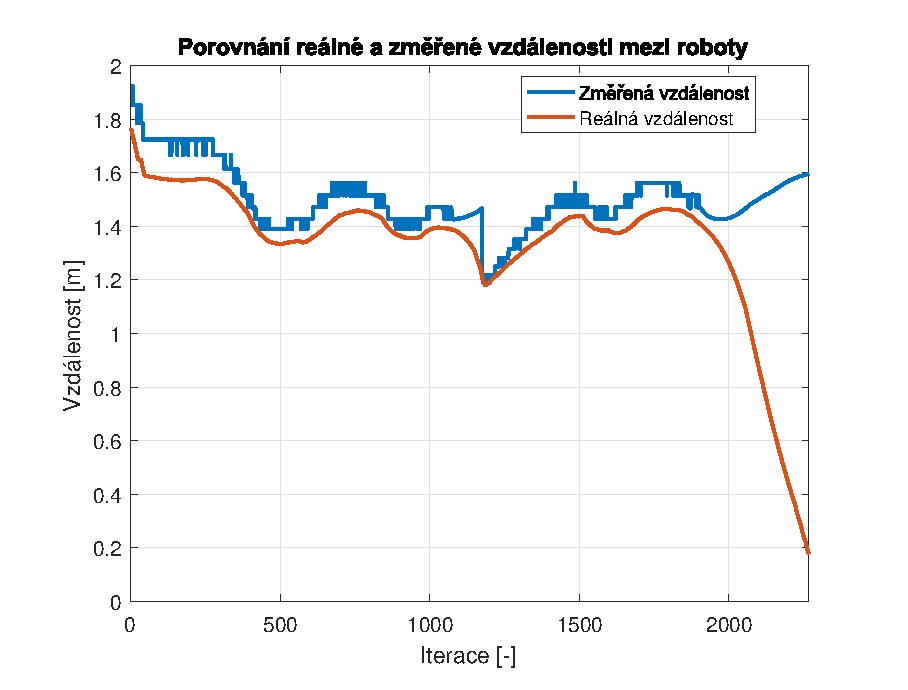
\includegraphics[width=0.8\textwidth]{images/5/dist.eps}
\end{figure}


\begin{figure}[hbt]
	\caption{Odchylka sledovaného objektu od středu kamery $\phi$}

	\label{odch}
	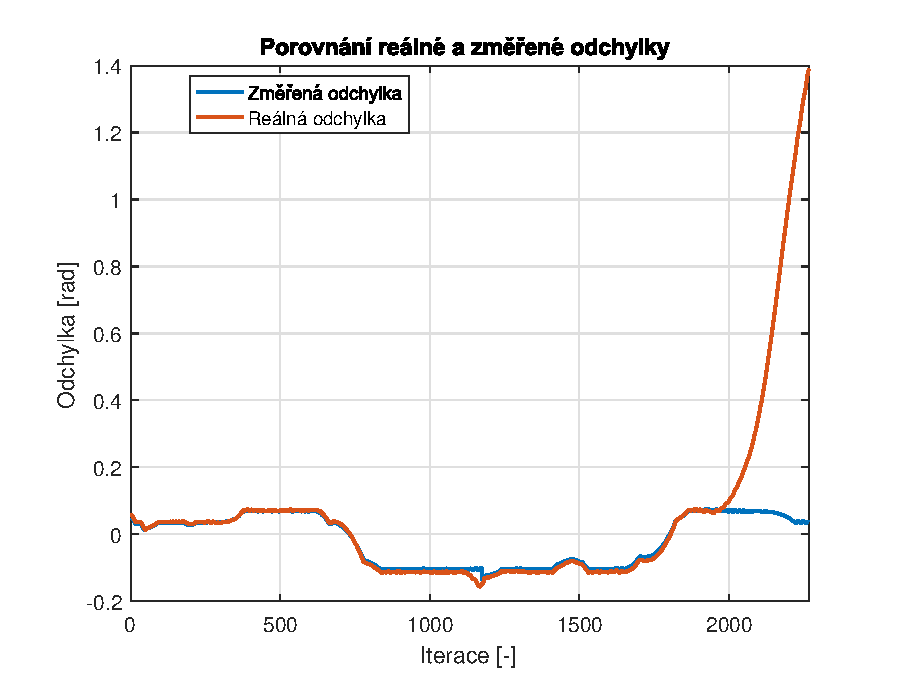
\includegraphics[width=0.8\textwidth]{images/5/odchylka.eps}
\end{figure}
Na obrázku \ref{dist} je také vidět, že změřená vzdálenost není stejná, jako reálná. Je to způsobeno nepřesnou kalibrací referenční vzdálenosti mezi následovaným a sledujícím robotem. Kdyby kalibrace byla přesnější, bylo by možné dosáhnout podobného výsledku, jako pro odchylku od středu kamery (viz obr. \ref{odch}), kde měření odpovídá reálné hodnotě.

\section{Měření polohy robotu}

\begin{figure}
	\caption{Poloha robotu během simulace}

	\label{rob_pos}
	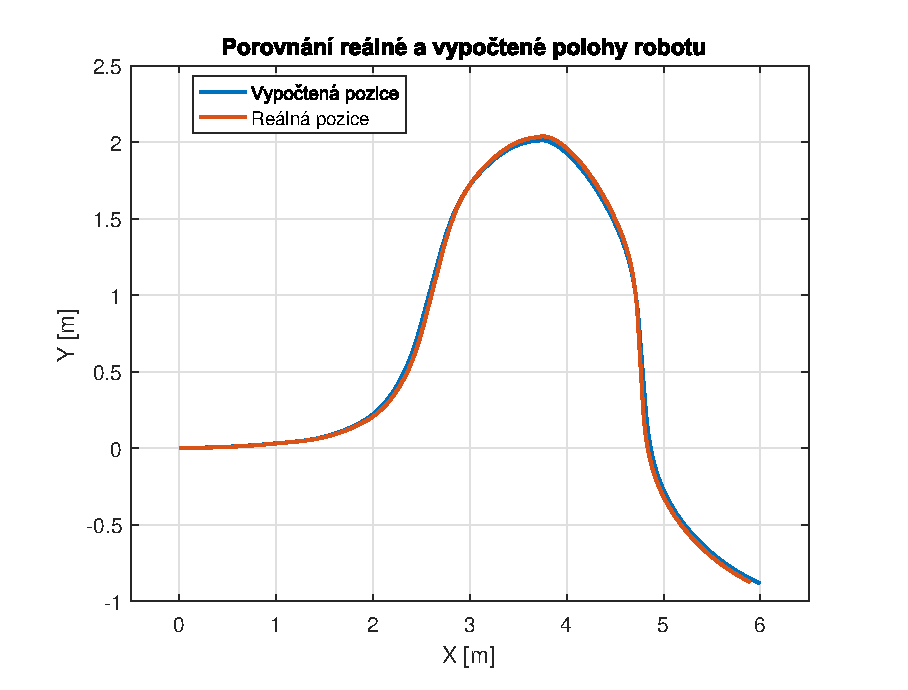
\includegraphics[width=0.8\textwidth]{images/5/pos_rob.eps}
\end{figure}

%https://chess.eecs.berkeley.edu/eecs149/documentation/differentialDrive.pdf
Jak bylo řečeno v \ref{kalman_section}, aby bylo možné spočítat polohu cíle vůči robotu, je třeba znát polohu robotu v globálních souřadnicích. Ačkoliv simulátor V-Rep nabízí možnosti pro přesné měření polohy objektů ve světových souřadnicích, v reálném světě tato možnost nemusí být použitelná, protože např. při navigaci robotu uvnitř budov nelze použít GPS. Proto byl v sekci \ref{ss_section} zaveden relativní souřadnicový systém, ve kterém se poloha robotu počítá. Pro toto měření lze v simulátoru odečítat vnitřní polohu rotačních kloubu robotu, na které jsou přidělány kola. V případě robotu s diferenciálním řízením, jeho pozici lze spočítat jako:

\begin{equation}
\begin{bmatrix}
x\\
y\\
h
\end{bmatrix} =
\begin{bmatrix}
x + \frac{(\Delta R + \Delta L)r_{k}}{2}\cos(h)\\
y + \frac{(\Delta R + \Delta L)r_{k}}{2}\sin(h)\\
h + \frac{(\Delta R - \Delta L)r_k}{2r_r}
\end{bmatrix},
\end{equation}

přičemž $\Delta L$ a $\Delta R$ značí změnu vnitřní polohy levého a pravého kloubů za čas $\Delta t$, $r_k$ je poloměr kola a $r_r$ je poloměr robotu, neboli polovina vzdálenosti mezi koly.

Porovnání reálné, tj. v simulátoru změřené, a vypočtené polohy robotu ve zvoleném souřadnicovém systému lze vidět na obrázku \ref{rob_pos}. Je patrné, že pro použitý typ robotu a relativní souřadnicovou soustavu je výpočet přesný a při použití přesných enkodérů lze tento výpočet aplikovat i na reálném robotu.

\section{Trajektorie robotu při jízdě s překážkami}

Po ověření funkčnosti detektorů a řízení robotu byl v simulátoru vytvořen model prostředí, ve kterém by robot měl sledovat člověka se značkou. Do scény byli umístěni i jiní lidé, a také různé překážky: kytka, stůl, strom, křeslo, sloup, jak je vidět na \ref{lidi}.
\begin{figure}[H]
	\caption{Simulace s člověkem a překážkami}

	\label{lidi}
	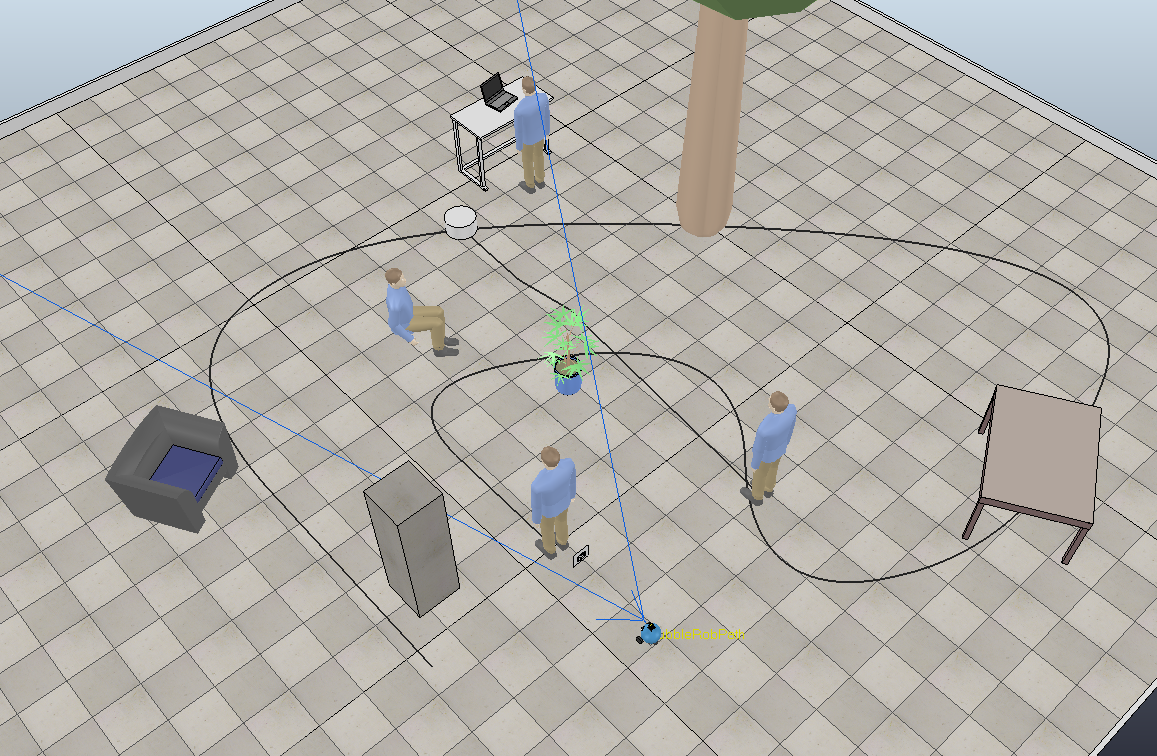
\includegraphics[width=0.9\textwidth]{images/5/people.png}
\end{figure}
Člověk měl předem definovanou cestu, kterou přesně dodržoval nehledě na překážky, proto procházel skrz ostatní objekty bez jakýchkoliv následků. Robot se ostatním objektům měl vyhýbat.

Trajektorie člověka a robotu jsou na obrázku \ref{trajektorie}. Šedě je na obrázku znázorněna kytka, zeleně strom a růžově kolemjdoucí, který během simulace přišel na uvedenou pozici. Jak je vidět, robot se snažil dodržovat trajektorii, podle které šel sledovaný člověk a přitom dokázal objíždět překážky, které mu v tom bránily. Nejproblematičtější část simulace byla na začátku, kdy člověk strmě zahnul doprava. V ten okamžik byla vizuální značka špatně detekovatelná, protože byla otočena vůči robotu téměř o 90$^\circ$. Navíc v určitém časovém intervalu byla značka skryta za listím, takže ji použitý algoritmus nedokázal najít ve snímku. Avšak tady je vidět, jak přínosné je použití Kalmanova filtru, který dokázal předpovědět na základě mála měření, kde se člověk nachází, proto ho robot rychle našel a sledoval i nadále.

\begin{figure}[H]
	\caption{Trajektorie robotu a člověka}

	\label{trajektorie}
	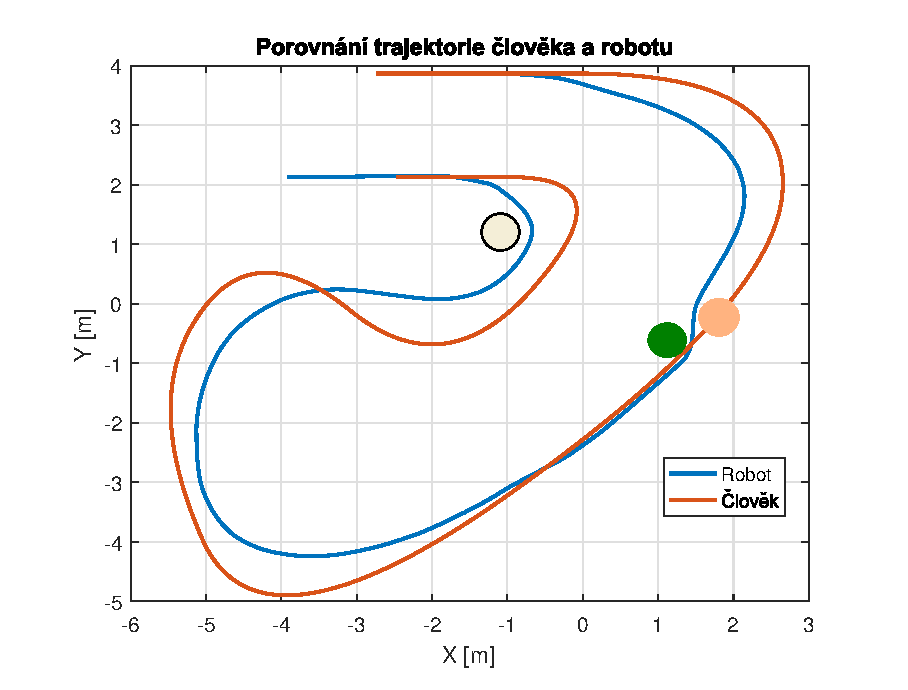
\includegraphics[width=0.8\textwidth]{images/5/trajek.eps}
\end{figure}
Dalším problematickým úsekem byla cesta mezi stromem a kolemjdoucím. Jelikož sledovaný člověk mohl procházet skrz objekty, došlo k tomu, že, když mu v cestě stal kolemjdoucí, prošel skrz něj a pokračoval dále. Značka tedy opět nebyla detekovatelná. Navíc mezi stromem a kolemjdoucím byl velice úzký průjezd a robot musel snížit rychlost, aby tam dokázal projet. Nakonec však robot nalezl sledovaného člověka a jel za nim až do konce simulace.
\chapter{Závěr}

Cílem této práce bylo navrhnout software pro autonomní řízení robotu následujícího člověka.

Pro detekci člověka v obrazu bylo rozhodnuto použit vizuální značku, která byla robotem známa, funkčnost takového řešení byla ověřena simulací. Robot dokáže spočítat vzdálenost a směr, ve kterém se detekovaná značka vůči němu nachází. Díky dálkoměru robot také ví, jestli na cestě k cíli jsou překážky. Pokud ano, pomocí Vector Field Histogram algoritmu je vypočten nový směr jízdy tak, aby robot nenarazil na žádnou překážku a zároveň byl co nejblíže člověku. Na základě spočtených parametrů se pomocí PID regulátoru vyhodnotí rychlosti, které je třeba aplikovat na motory, aby robot dosáhl cílové pozice vůči sledovanému člověku. Navíc pro případ, kdy robot nedetekuje značku, a tedy ani nedokáže spočítat vzdálenost k cíli, je použit Kalmanův filtr, který předpovídá polohu cíle na základě předchozích měření.

V simulátoru bylo provedeno několik testů s roboty, nastavení simulací a výsledky některých testů jsou popsány v kapitole \ref{simulace}. Průměrná vzdálenost $d$ mezi roboty byla \SI{1.99}{\meter} a odchylka sledovaného robotu od středu kamery $\phi$ stanovila \SI{0.0023}{\radian}. Jelikož rychlost robotů byla stejná a počáteční vzdálenost mezi nimi byla \SI{2}{\meter}, sledující robot se nedokázal přiblížit referenční hodnotě \SI{1}{\meter}. Dále pak byla změřena průměrná absolutní odchylka mezi reálnou a vypočtenou polohou sledujícího robotu, která stanovila \SI{0.17}{\meter}. Rozdíl mezi reálnou a spočtenou hodnotou směru jízdy robotu byla \SI{-0.02}{\radian}. Nakonec byl spočítán rozdíl mezi reálnou a vypočtenou pomocí Kalmanova filtru polohou sledovaného robotu, ten stanovil \SI{0.32}{\meter}. Tak velká odchylka byla způsobena tím, že byly simulovány situace, kdy značka zmizí ze zorného pole robotu. Avšak robot dokázal pokaždé najít značku znovu a pokračovat v jízdě. 


Tato práce byla velkým přínosem hlavně proto, že v ní byla možnost vyzkoušet různé techniky používané pro řízení mobilních robotů. Navíc díky této práci jsme se seznámili s simulačními prostředí pro robotiku a OpenCV knihovnou, která je běžně používána pro implementaci softwaru pro počítačové vidění a strojové učení.


\appendix

\chapter{Přehled algoritmů pro vyhýbání se překážkám}
\label{obstacle_avoidance}
\begin{figure}[H]
	\caption{Souhrn algoritmů pro vyhýbání se překážkám \cite[s. 287--290]{cite:20}}
	\label{korelace}
	\subfloat{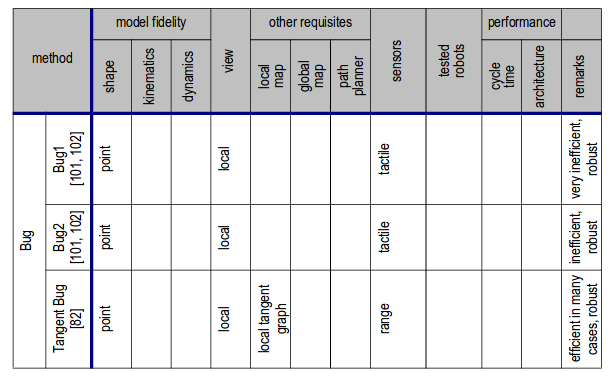
\includegraphics[width=1\textwidth]{images/6/4.png}}
	\newline
\end{figure}
\begin{figure}[H]\ContinuedFloat
		\caption{Souhrn algoritmů pro vyhýbání se překážkám \cite[s. 287--290]{cite:20}}
	\subfloat{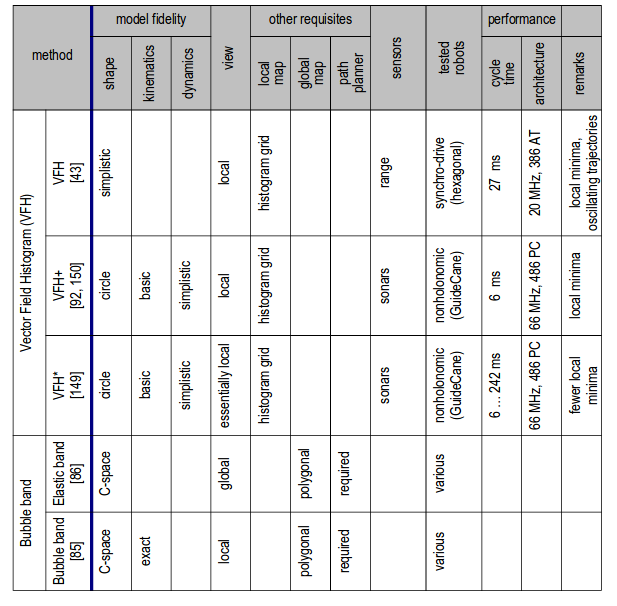
\includegraphics[width=1\textwidth]{images/6/1.png}}
	\newline
\end{figure}
\begin{figure}[H]\ContinuedFloat
		\caption{Souhrn algoritmů pro vyhýbání se překážkám \cite[s. 287--290]{cite:20}}
	\subfloat{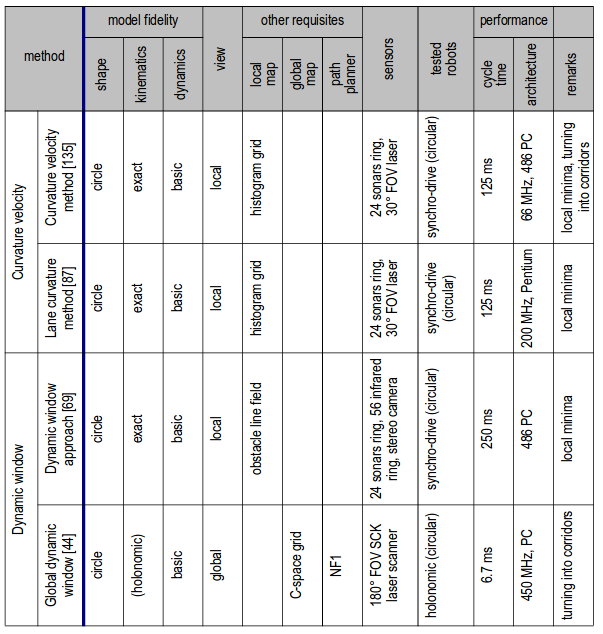
\includegraphics[width=1\textwidth]{images/6/2.png}}
	\newline
\end{figure}
\begin{figure}[H]\ContinuedFloat	
	\caption{Souhrn algoritmů pro vyhýbání se překážkám \cite[s. 287--290]{cite:20}}
	\subfloat{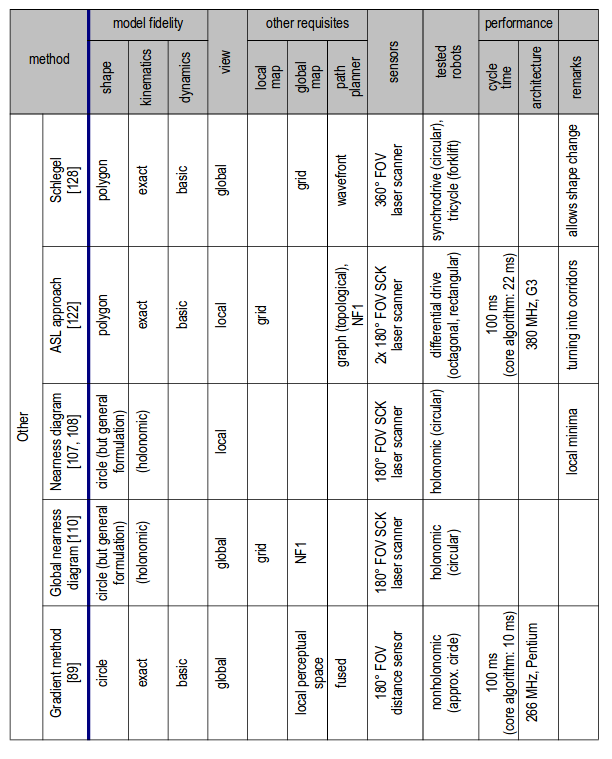
\includegraphics[width=1\textwidth]{images/6/3.png}}
	\newline
\end{figure}
\printindex

\bibliographystyle{unsrt}
\bibliography{ctutest}


\end{document}
